\section{Results}

\subsection{Network Benchmarks}

\begin{figure*}
	\centering
	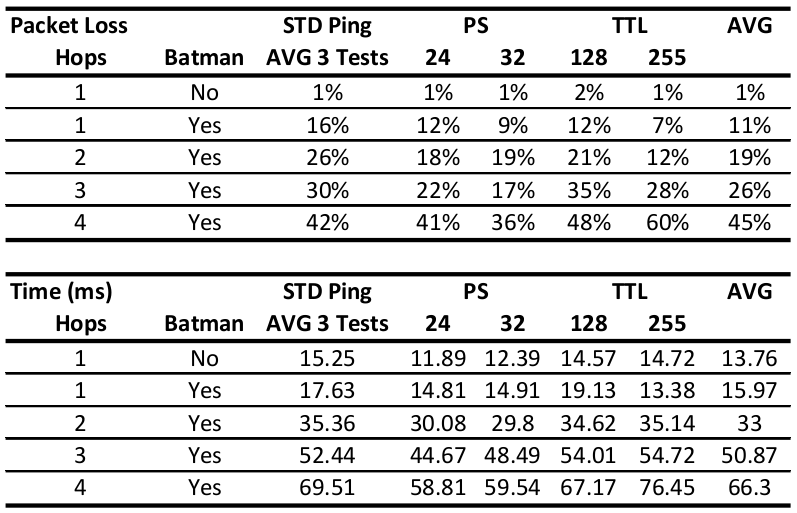
\includegraphics[scale=0.4]{902sheet}
	\caption{The data received from operating at 902/915 MHz.}
	\label{fig:spreadhsheet2}
\end{figure*}

\begin{figure*}
	\centering
	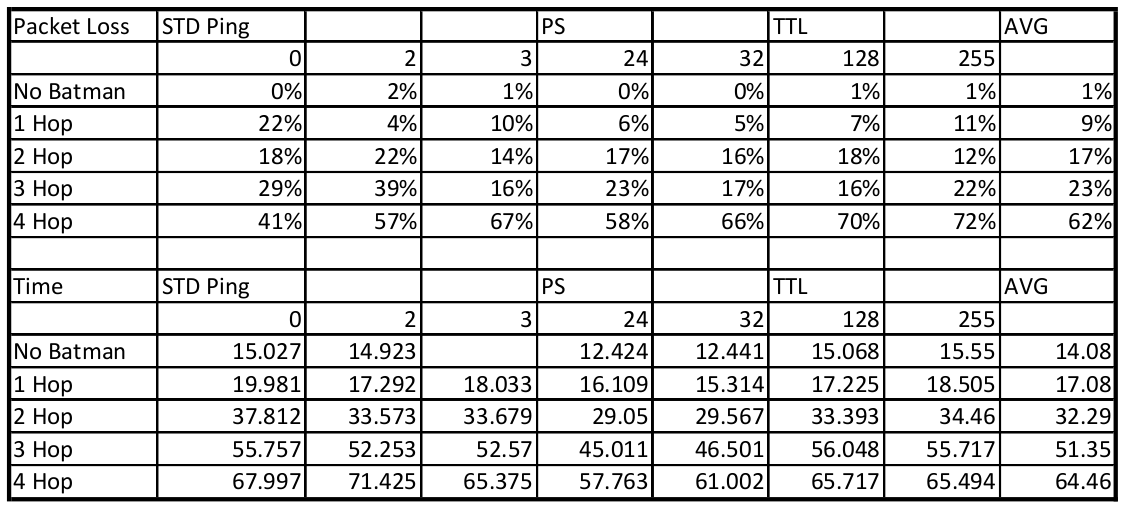
\includegraphics[scale=0.4]{2400}
	\caption{The data received from operating at 2.4/2.5 GHz.}
	\label{fig:2400}
\end{figure*}

\begin{figure}
	\centering
	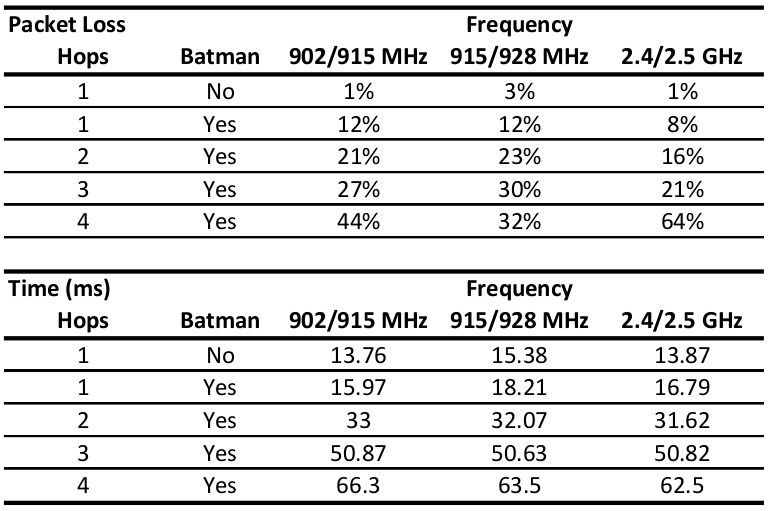
\includegraphics[scale=0.4]{alldata}
	\caption{The Averages from all three tests.}
	\label{fig:alldata}
\end{figure}


\subsection{Route Changes}

\begin{figure*}
	\centering
	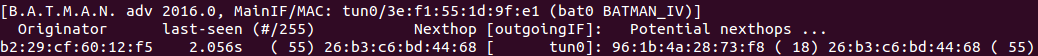
\includegraphics[scale=0.5]{2PotentialHops}
	\caption{The initial condition, where there are two possible routes the packet can take.}
	\label{fig:2Hops}
\end{figure*}

\begin{figure*}
	\centering
	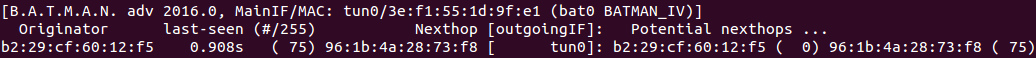
\includegraphics[scale=0.5]{hopchange}
	\caption{After the gain is reduced, the packets are now routing through a different node.}
	\label{fig:NewHop}
\end{figure*}

\subsection{Frequency Changes}

\begin{figure}
	\centering
	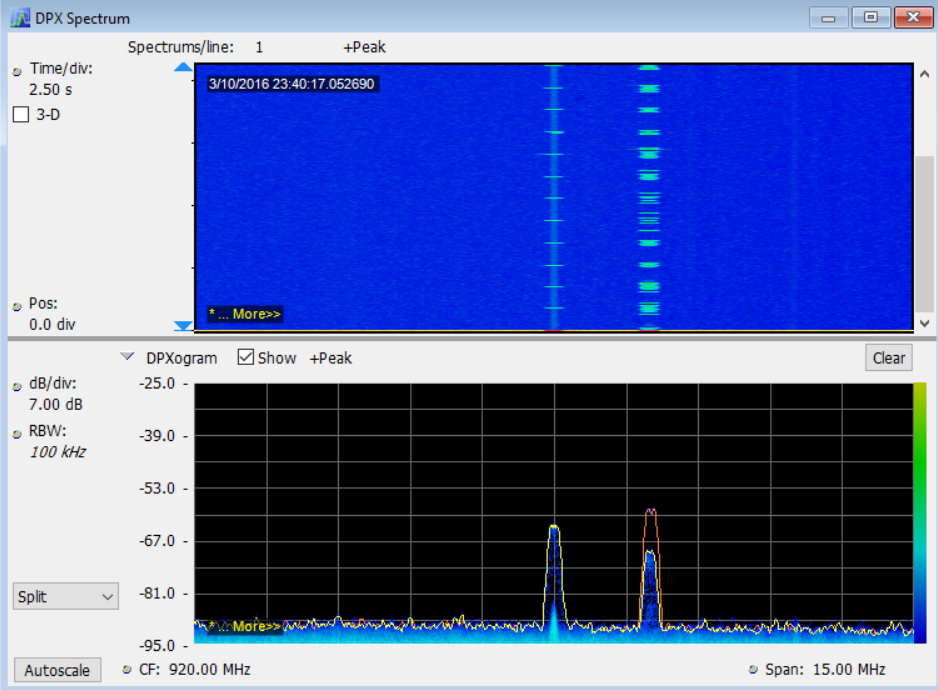
\includegraphics[scale=0.4]{FrequencyShift922-920}
	\caption{The result of using ALFRED to shift frequencies. One Node is left behind as the others move to the new channel.}
	\label{fig:freqshift}
\end{figure}


